\chapter{Реализация Allure Framework} 
\label{chapter3}

\section{Общая схема работы} 

Общая схема работы фремворка показана на рисунке \ref{fig:allure}. Рассмотрим подробнее назначение отдельных частей.

\begin{figure}[htb]
\centering
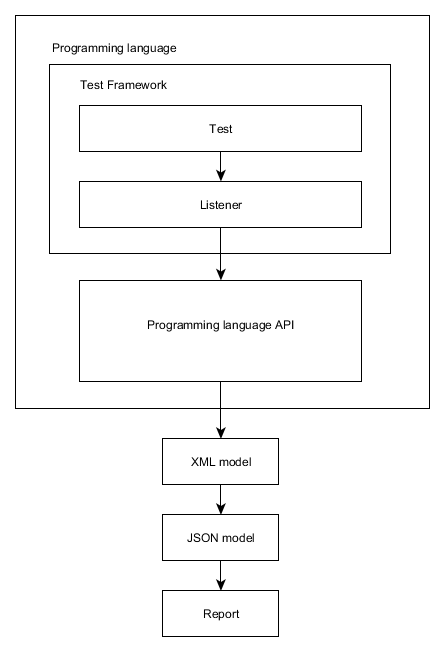
\includegraphics[height=160mm]{structure.png}
\caption{Общая схема фремворка Allure}
\label{fig:allure}
\end{figure}

\subsection{Listener}

Для большинства тестовых фремворков xUnit есть возможность подключить листенер для сбора информации о ходе тестов. Мало того, подключение листенера, как правило, вынесено на уровень конфигурации запуска, что полностью удавлетворяет требованиям работы. Для адаптации тестового фремворка достаточно реализовать тест листенер используя соответсвующее API языка программирования.

Однако стоит заметить, что не всю необходимую информацию о ходе теста можно собрать используя листенер, так как он оперирует терминологией xUnit. Сбор остальной информации о тестах, например информацию о пройденных шагах и сделанных аттачментах, будет реализован на уровне API языка программирования.

\subsection{Programming language API}

API для языка программирования представляет из себя набор обработчиков событий и сами события, используя которые можно полностью описать жизненный цикл теста. Программный инетрфейс содержит в себе следующие события:

\begin{itemize}
\item начало/конец тестового запуска;
\item начало/конец тест суита;
\item начало/конец тест кейса;
\item начало/конец шага;
\item сохранение аттачмента;
\item добавление параметров запуска/тест суита/тест кейса;
\item изменение статуса теста/шага;
\item добавление пометок к тесту.
\end{itemize}

С использованием API для языка программирования сильно упрощается написание и поддержка листнеров для тестовых фремворков. Вся собранная информация о ходе тестов сохраняется в XML модель. 

\subsection{XML model}

Собранная о тесте информация серелизуется в виде XML файлов. Для каждого теста создается свой файл. Сохраняются только те данные, которые нельзя синтезировать, что упрощает реализацию и поддержку интерфейса для языка программирования. Простейший пример сохранненной информации об одном тесте:

\begin{lstlisting}[style=XML]
<?xml version="1.0" encoding="UTF-8" standalone="yes"?>
<ns2:test-suite xmlns:ns2="urn:model.allure.qatools.yandex.ru" start="1400681607876" stop="1400681627123">
    <name>my.company.SampleTest</name>
    <test-cases>
        <test-case start="1400681608883" stop="1400681608891" status="passed">
            <name>test_pass</name>
        </test-case>
    </test-cases>
    <labels/>
</ns2:test-suite>
\end{lstlisting}

\subsection{JSON model}

На следующем этапе данные конвертируются в более удобный для оборажения формат. Более подробно данный уровень будет рассмотрен в следующих главах.

\subsection{Report}

Отображает результаты разными способами. Более подробно будет рассмотрен в следющих главах.

\section{Анализ предыдущих разработок}

Еще написания автором работы существовали некторые наработки, которые похволяли строить отчет. Но не существовало единого и универсального отчета, так как все наработки писались под конкретные задачи. Их главный недостаток - данные отчеты подходили только для отображения резульатов специфичных тестов. Также важными недостатками являлись сложность подключения данных отчетов к тестам, невозможность использовать отчет с разными тестовыми фремворками. 

\section{xUnit}

На данный момент xUnit является стандартом в тестировании. Для большинства современных языков программирования есть реализатция тестового xUnit фремворка. При разработке фремворка автор опирался в основном на этот стандарт. Рассмотрим подробнее, что такое xUnit.

Во всех реализация xUnit предоставляется базовый набор функций, которые позволяют решать следующие задачи:

\begin{itemize}
\item описывать тест как тестовый метод (Test Method);
\item описывать ожидаемые результаты внутри тестового метода в форме вызовов методов с утверждением (Assertion Method);
\item аггрегировать тесты в наборы, которые могут запускаться с помощью одной команды;
\item запускать один или несколько тестов для получения отчета о результатах запуска.
\end{itemize}

Автор данной работы изначально планировал расширить стандартную модель xUnit, добавив в нее свои поля, тем самым сразу обеспечив совместимость со всеми xUnit фреймворками. Однако в ходе разработки стало понятно, что в той модели, которую предоставляет xUnit есть существенные недостатки, и было решно создать модель, похожую на xUnit, но лишенную этих недостатков. 

\section{Сценарий теста}

Не всегда те люди, которые анализируют результаты тестирования пишут тесты. Особенно часто это бывает в больших компиниях, когда количество тестов велико. И в таких случаях, для того, чтобы понять, что конкретно делал тест, надо знать его сценарий. Для этого тест разбивается на шаги, информация о которых добавляется в отчет. Также такой подход помогает локализовать проблему - ведь высокоуровневые тесты часто делают большое количество проверок.

\newpage
\section{Примеры работы фреймворка Allure для JUnit тестов}

Одно из основных достоинств разработаного автором фреймворка является прозрачная интеграция с существующими тестовыми системами. Рассмотрим простейший JUnit тест:
Зачастую, это 

 
\begin{lstlisting}
public class SimpleTest {

    @Test
    public void simpleTest() throws Exception {
        assertThat(4, is(2 + 2));
    }
    
    public int sum(int a, int b) {
		return a + b;
	}    
    
    public void check(int a, int b, int c) {
    	assertThat(c, is(a + b));	
    }
}
\end{lstlisting}

Для данного теста уже можно построить отчет. Например, если тест запускается с помощью Maven, достаточно добавить конфигурацию [ссылка на приложение] в pom.xml проекта. Отчет, построенный для данного теста будет похож на стандартный отчет surefire. 

Для того, чтобы отобразить информацию о тестовом сценарии достаточно проаннотировать соответствующие методы аннотацией @Step.

\begin{lstlisting}
public class SimpleTest {

    @Test
    public void simpleTest() throws Exception {
        int c = sum(2, 2);
        check(2, 2, c);
    }
    
    @Step("Считаем сумму '{0}' и '{1}'")
    public int sum(int a, int b) {
		return a + b;
	}    
    
    @Step("Проверяем, что сумма '{0}' и '{1}' равна '{c}'")
    public void check(int a, int b, int c) {
    	assertThat(c, is(a + b));	
    }
}
\end{lstlisting}

Так же просто мы может добавлять к тесту аттачменты, указывать параметры, группировать тесты по требованиям и историям, и так далее.


В предыдущих главах были подробно описаны концепции положенные в основу фремворка Allure. В этой главе
описаны технические подробности реализации.

\section{Подключение к тестам}

Информацию, которую фремворк собирает о тестах, можно разделить на две группы:

\begin{itemize}
\item информация, которую можно получить, не меняя код тестов, например, имя теста, статус выполнения и время выполнения теста;
\item та информация, которую будет предоставлять тестировщик. Например, сценарий теста, описание теста и требования к тесту.
\end{itemize}

Большинство фремворков xUnit предоставляют интерфейс листенера, позволяющий собирать первый тип информации. Данный подход полностью удовлетворяет требованиям, так как подключение листенеров в большинстве случаев вынесено на уровень конфигурации запуска тестов.

Со вторым типом информации намного интереснее. В качестве примера рассмотрим реализацию для jUnit.

\subsection{Шаги}

В языке программирования Java шаг теста это любой метод, аннотированный аннотацией @Step. Для того, чтобы собрать информацию о пройденных шагах, надо выполнять некоторый код до и после каждого вызова такого метода. Автор воспользовался фреймворком AspectJ для решения этой задачи. Данный фремворк позволяет налету модифицировать байт-код классов во время их загрузки в JVM. Для того, чтобы "подцепиться" к нужным нам методам, надо описать точки входа (pointcuts) и аспекты (aspects): 

\begin{lstlisting}
@Pointcut("@annotation(ru.yandex.qatools.allure.annotations.Step)")
public void withStepAnnotation() {
    //pointcut body, should be empty
}

@Pointcut("execution(* *(..))")
public void anyMethod() {
    //pointcut body, should be empty
}

@Before("anyMethod() && withStepAnnotation()")
public void stepStart(JoinPoint joinPoint) {
    ...
}

@AfterThrowing(pointcut = "anyMethod() && withStepAnnotation()", throwing = "e")
public void stepFailed(JoinPoint joinPoint, Throwable e) {
    ...
}

@AfterReturning(pointcut = "anyMethod() && withStepAnnotation()", returning = "result")
public void stepStop(JoinPoint joinPoint, Object result) {
    ...
}
\end{lstlisting}

